\documentclass{VUMIFPSkursinis}
\usepackage{algorithmicx}
\usepackage{algorithm}
\usepackage{algpseudocode}
\usepackage{amsfonts}
\usepackage{amsmath}
\usepackage{bm}
\usepackage{caption}
\usepackage{color}
\usepackage{float}
\usepackage{graphicx}
\usepackage{listings}
\usepackage{subfig}
\usepackage{wrapfig}
\usepackage{enumitem}
\usepackage[utf8]{inputenc}
%\usepackage{enumerate}

%PAKEISTA, tarpai tarp sąrašo elementų
\setitemize{noitemsep,topsep=0pt,parsep=0pt,partopsep=0pt}
\setenumerate{noitemsep,topsep=0pt,parsep=0pt,partopsep=0pt}

% Titulinio aprašas
\university{Vilniaus universitetas}
\faculty{Matematikos ir informatikos fakultetas}
\department{Programų sistemos}
\papertype{Laboratorinis darbas}
\title{Kelionių į Mėnulį maršrutų planavimo programa „Poon“}
\status{3 kurso 5 grupės studentai}
\author{Gabrielė Žielytė}
\secondauthor {Daumantas Šimkus}
\thirdauthor {Nedas Valentinovičius}
\titleineng{}

\date{Vilnius – \the\year, Galutinė versija}

% Nustatymai
\setmainfont{Palemonas}   % Pakeisti teksto šriftą į Palemonas (turi būti įdiegtas sistemoje)
\bibliography{bibliografija}

\begin{document}
	
% PAKEISTA	
\maketitle

%TURINYS
\thispagestyle{empty}
\tableofcontents


\sectionnonumnocontent{Anotacija}
Šiame dokumente aprašoma bilietų pirkimo kelionėms į mėnulį telefoninė programa „Poon“. Darbo tikslas - sukurti patogią, vartotojui suprantamą ir intuityvią vartotojo sąsają.
Studentų, dirbusių prie šio projekto, kontaktai bei indėlis:
\begin{itemize}
\item Gabrielė Žielytė - gabriele.zielyte@mif.stud.vu.lt. Atsakinga už įkvepiančias dizaino idėjas, jų susiejimą su siekiais, suinteresuotųjų bei jų lukesčių identifikavimą.
\item Daumantas Šimkus - daumantas.simkus@mif.stud.vu.lt. Atsakingas už esamų veiklų aprašus, būsimuosius scenarijus, vartotojų poreikius, naudotojų veiklų charakteristikas.
\item Nedas Valentinovičius - nedas.valentinovicius@mif.stud.vu.lt. Atsakingas už dokumento struktūrą, įvadą, suinteresuotųjų identifikavimą, esamų veiklų aprašymą, poreikius, panaudojamumo siekius bei būsimuosius scenarijus.
\end{itemize}
\thispagestyle{empty}

\cleardoublepage\pagenumbering{arabic}
\setcounter{page}{4}

\section{Įvadas}
\textbf{Programų sistemos pavadinimas: } Kelionių į Mėnulį maršrutų planavimo programa „Poon“
\bigskip

\textbf{Trumpasis pavadinimas: } „Poon“
\bigskip




\textbf{Projekto aprašas: } Kelionėms į Mėnulį tapus realybe, tapo ypač svarbu tvarkinga, aiški, moderni ir svarbiausia saugi kelionių planavimo sistema. Į Mėnulį plūsta žmonės iš skirtingų kultūrų, tikėjimo, puoselėjantys įvairias vertybes. Todėl Poon misija yra gerbti kiekvieną norintįjį skristi, parūpinti jam saugią ir malonią aplinką su kuo aiškesnėmis taisyklėmis kelionėms tarp Žemės ir Mėnulio.

\bigskip
\textbf{Sprendžiamos problemos: }
\begin{enumerate}
\item Šiuo metu bilietai į Mėnulį perkami individualiai iš skrydžio kompanijų, o „Poon“ sistema jas visas apjungs.
\item Maršrutų patikrinimas ir bilietų pirkimas yra atskiri veiksmai, kuriuos ši programa apjungia į vieną vartotojo sąsają
\item Netikslūs, su skryžių kompanijomis nesusinchronizavę maršrutų tvarkaraščių puslapiai klaidina vartotojus, o „Poon“ programoje matomi tvarkaraščiai bus sinchronizuojami tiesiogiai su skrydžių bendrovėmis.
\item Šiuo metu kelių bilietų pirkimas yra itin komplikuotas, o „Poon“ programoje tai bus taip pat paprasta, kaip pirkti vieną bilietą.
\item Nėra galimybės iškart užsisakyti bilietą atgal, tačiau ši programa išsprendžia šią problemą iškart siūlydama įsigyti bilietus atgal su bet kuria atgal parskraidinti galinčia skrydžių kompanija.
\item Nėra patogios statistikos apie kiekvieną skrydžių kompaniją. „Poon“ anonimiškai ves statistiką ir ja dalinsis su visu pasauliu, kad būtų aiškiai matomi skirtingų skrydžių bendrovių populiarumai tarp vartotojų.
\end{enumerate}

\section{Suinteresuotieji}
Šio skyriaus tikslas yra išskirti suinteresuotųjų asmenų grupes tam, kad būtų galima nustatyti, kokie funkcionalumai yra reikalingi, kokie tiksliai yra naudotojų poreikiai, kam ši sistema bus naudingiausia bei atsižvelgti į konkurentų sistemas, jų neišnaudotas galimybes bei galimas tobulintinas sritis.

Programos savininko lūkestis yra sukurti nagrinėjamoms suinteresuotųjų grupės patogią vartotojo sąsają, supaprastinančią bilietų i Mėnulį pirkimą. Ši programa nesiekia pelno, tačiau naudojamų pagalbinių sistemų (duomenu bazių, statistikos saugojimo paslaugų) išlaidoms padengti vartotojams rodomos naudojimui netrukdančios reklamos.

\subsection{Pirminiai} 
Šios programos pirminiai suinteresuotieji yra \textbf{pilnamečiai asmenys, norintys planuoti keliones į Mėnulį}. Kadangi pasaulio valstybėse pilnametystė yra reglamentuota skirtingai. Poon pilnametis asmuo yra tas, kuris pagal savo valstybės įstatymus, pilnai atsako už save. Pavyzdys būtų mokslinius tyrimus atliekantys asmenys. Kadangi skrydžiai į Mėnulį įprastu dalyku tapo neseniai, šis dangaus kūnas vis dar traukia mokslininkus bei tyrinėtojus. Programa, leidžianti užsisakyti bilietus tiek šiandien, tiek už mėnesio vykstantiems skrydžiams labai praverstų staiga į tyrimų stotį norintiems skristi ar po kurio laiko vykstančius tyrimus planuojantiems mokslininkams. 

Pirminių suinteresuotųjų esminiai lūkesčiai būtų:
\begin{enumerate}
\item Aiškus ir greitas skrydžių pasirinkimas \label{itm:aisku}
\item Lengva apmokėjimo sistema\label{itm:apmokejimas}
\item Galimybė bilietus saugoti ilgą laiką\label{itm:saugoti}
\item Gebėjimas bilietus perduoti kitiems asmenims\label{itm:perduoti}
\item Pigių skrydžių radimas\label{itm:pigu}
\end{enumerate}

\subsection{Antriniai} 
Antriniai šios programos suinteresuotieji yra \textbf{statistinių analizių vedėjai}. Ši suinteresuotųjų grupė naudosis mūsų programos pateikiamomis statistikomis tam, kad galėtų gauti tikslią bei visas skrydžių įmones apimančią statistiką. Šiai grupei svarbu žinoti, kiek mėnesinių klientų turi skirtingos skrydžių kompanijos, kurie skrydžiai populiariausi ir panašias statistikas, kurias „Poon“ programa ves.

Antrinių suinteresuotųjų esminiai lūkesčiai būtų:
\begin{enumerate}
\item Tiksli bei aiški statistinė skrydžų analizė\label{itm:analize}
\item Duomenų anonimiškumas\label{itm:anonim}
\end{enumerate}

\subsection{Tretiniai} Tretiniai suinteresuotieji būtų šios \textbf{sistemos konkurentai}, nes jų veiklą veikia šios sistemos sėkmė arba nesėkmė. Šiuo metu rinkoje egzistuoja ne viena kompanija, organizuojanti skrydžius į Mėnulį. Kiekviena iš jų turi savą bilietų pirkimo sistemą, kur galima nusipirkti tik vienos skrydžių kompanijos bilietus, taip pat kiekviena naudojasi skirtinga mokėjimo sistema, o tai kelia vartotojams daug bėdų, ypač kai ilgą laiką buvo naudojamasi vienos kompanijos paslaugomis ir yra nuspręsta pradėti naudotis kitos kompanijos siūlomais skrydžiais. 

Konkretūs "Poon" konkurentų pavyzdžiai būtų "Comet express" ir "PlanetStar". Šios sistemos turi kelias neišnaudotas galimybės, kurias „Poon“ sieks pagerinti ir implementuoti į savąją sitema:
\begin{enumerate}
\item Konkurentų programos leidžia nusipirkti tik jų kompanijos bilietus, todėl bilietų ir datų skaičius yra gana ribotas
\item Jų vartotojo sąsajos atrodo ir yra naudojamos skirtingai, o „Poon“ sistemos sąsają bus galima naudoti prikti bilietus iš abiejų kompanijų
\item Programos savo statistikas viešina tik kartą per pusmetį, o „Poon“ sistemos teikiami duomenys bus matomi nuolatos.
\end{enumerate}

Poon bus primoji programa, leidžianti pirkti bilietus iš visų didžiųjų skrydžių organizatorių bei leidžianti susimokėti visais pagrindiniais mokėjimo būdais. Tai išspręs didžiąją dalį problemų, šiuo metu kylančių noritintiems skristi į Mėnulį asmenims, bei maždaug 15\% sumažins "Comet express" ir "PlanetStar" skrydžių planavimo sistemų vartotojų kiekį, nes didelė dalis vartotojų neabejotinai pradės naudoti daug patogesnę bei intuityvesnę „Poon“

\subsection{Kiti}
Kiti suinteresuotieji yra sistemos projektuotuojai, realizuotojai bei palaikytojai. Kiekviena žmonių grupė prie sistemos gerovės prisidės tokiais būdais:
\begin{enumerate}
\item Sistemos projektuotojai bei programuotojai Nedas Valentinovičius, Gabrielė Žielytė bei Daumantas Šimkus suprojektuos bei suprogramuos kitoms vartotojų grupėms patogią bei funkcionalią vartotojo sąsają.
\item Naudojamos duomenų bazės administratoriai užtikrins nuolatinį saugomų duomenų prieinamumą.
\item Statistinių duomenų centro darbuotojai užtikrins, kad „Poon“ vedami duomenys nėra klastojami bei tikslūs.
\end{enumerate}

\section{Keliautojų poreikiai}
Šiame skyriuje bus pateikiama detali keliautojų poreikių, siekių ir kitų tikslų analizė.

\subsection{Einamųjų veiklų analizė}
Toliau bus pateiktos kelios einamosios veiklos, analizuojamai naudotojų grupei keliančios nepatogumus.

\subsubsection{Pirma kompiuterizuojama veikla}
[TRUMPAS VIENO SAKINIO SCENARIJUAUS APRAŠYMAS]

\textit{TAS BLOGAS NAUDOJIMO SCENARIJUS, ŠIUO METU KELIANTIS ŽMOGUI PROBLEMAS}

Pateiktame apraše išdėstytos esamos veiklos problemos ir neišnaudotos galimybės:  
\begin{itemize}
\item ČIA SURAŠOMOS VISOS TOS PROBLEMOS, KURIOS MATOMOS SCENARIJUJE
\end{itemize}

\subsubsection{Antra kompiuterizuojama veikla}
Aprašoma į darbą skubančio žmogaus bilietų pirkimo procedūra: 

\textit{Alisa skubėdama į darbą telefonu perka bilietus skrydžiui į Mėnulį, kuris vyks kitos dienos vakare. Telefone ji atsidaro „PlanetStar“ programėlę, kurioje pamato, kad įios kompanijos skrydžių bilietai tam reisui yra išpirkti. Tuomet ji atsidaro „Comet Express“ programėlę, kurioje įsigyja bilietą, kuris yra išsaugomas pačioje programėlėje. Tuomet Alisa vėl atsidaro pirkimų langą, ir susiranda skrydį atgal iš Mėnulio į Žemę. Ji vėl atlieka visą pirkimo procedūrą ir išsisaugo bilietą.}

Pateiktame apraše išdėstytos esamos veiklos problemos ir neišnaudotos galimybės:  
\begin{itemize}
\item Tenka naudotis keliomis sistemomis, kad rasti patogius skrydžių laikus
\item Įsigyti bilietai yra išsaugomi pačioje programėlėje, kurioje jie buvo pirkti. Vartotojui neduodamas pasirinkimas, kur norėtų juos išsisaugoti
\item Nepasiūloma iškart įsigyti bilietus skrydžiui atgal, tenka iš naujo atlikti visą pirkimo procedūrą.
\end{itemize}

\subsubsection{Trecia kompiuterizuojama veikla - JEI TOKIA YRA. SITAS VIS KARTOJAMAS BLOKAS}
[TRUMPAS VIENO SAKINIO SCENARIJUAUS APRAŠYMAS]

\textit{KITAS BLOGAS NAUDOJIMO SCENARIJUS, ŠIUO METU KELIANTIS ŽMOGUI PROBLEMAS}

Pateiktame apraše išdėstytos esamos veiklos problemos ir neišnaudotos galimybės:  
\begin{itemize}
\item ČIA SURAŠOMOS VISOS TOS PROBLEMOS, KURIOS MATOMOS SCENARIJUJE
\end{itemize}

\subsubsection{Naudotojų ir veiklų charakteristikos}
\textbf{Alisos charakteristikos: } Pavyzdiniame scenarijuje Alisa yra gerai įvaldžiusi mobilųjį prietaisą, supranta, kaip reikia pirkti bilietus įvairiose sistemose. Taigi ji yra gerai patyrusi tokių sistemų naudotoja. Jos motyvacija yra greitai ir be nesklandumų įsigyti bilietus, nes suprantama, kad skrydžių į Mėnulį paslaugomis ji naudojasi dažnai. Demografinės charakteristikos nenurodytos, tačiau galima jį priskirti jaunam ar vidutiniam amžiui, kai speciali parama nereikalinga. 

Veiklos dažnis: bilietų pirkimas yra itin dažnas veiksmas, ypač dirbantiems žmonėms. Šį veiksmą jie atlieka kelis kartus per savaitę, todėl svarbu pirkimo procesą padaryti paprastą ir prieinamą visiems vartotojams.

Veiklos trukmė: bilietu pirkimas viduriniškai užtrunka apie 10 minučių. Ši veikla yra vykdoma nuosekliai bei individualiai.

Veiklos aplinka: aprašytame scenarijuje Alisa judėjo, aktyviai skubėjo į darbą, todėl aplinka yra nerami.

\subsection{Būsimieji panaudojimo scenarijai}
Toliau bus pateikti keli pavyzdiniai panaudojimo scenarijai, kurie padės išspręsti vartotojams kylančias problemas

\subsubsection{Pirmasis scenarijus}
Scenarijus, aprašantis paprasto pirkimo procesą, kuriame vartotojas su draugu nori skristi į mėnulį šios dienos pabaigoje

\begin{enumerate}
\item Vartotojas pagrindiniame meniu pasirenka pasirinkima „Pirkti bilietus“
\item Vartotojas supildo informaciją apie skrydį.
\begin{enumerate}[label*=\arabic*.]
\item Pažymi, jog skris du žmonės.
\item Pažymi, jog skris tik į vieną pusę.
\item Pasirenka, jog skris iš Žemės.
\item Pasirenka, jog išvykti nori šiandien po 18:00 val.
\end{enumerate}
\item  Sistema pateikia sąrašą skrydžių, kurie vyksta iš Žemės ir kurių išvykimo laikas yra ne ankstesnis nei nurodyta vartotojo ir turi bent dvi laisvas vietas. Prie kiekvieno skrydžio yra nurodyta kaina.
\item Vartotojas pasirenką norimą skrydį.
\item Sistema parodo to skrydžio išvykimo ir atvykimo datas su planuojamais laikais, skrydžio kainą bei galimas sėdimas vietas.
\item Vartotojas pasirenka sėdimas vietas ir spaudžia mokėti.
\begin{enumerate}[label*=\arabic*.]
\item Vartotojas suveda asmens dokumento duomenis.
\item Įveda elektroninio pašto adresą.
\item Pasirenka apmokėjimo būdą.
\item Susimoka už kelionę.
\end{enumerate}
\item Sumokėjus sistema išsiunčia bilietus į el.paštą.
\item Vartotojas viena iš bilietų persiunčia draugui.
\end{enumerate}

\subsubsection{Antrasis scenarijus}
Scenarijus, aprašantis sistemos paruošimą bei naudojimą žmonėms su negalia
\begin{enumerate}
\item Atsisiuntus programą, vartotojui leidžiama tiek balsu, tiek paspaudimu pasirinkti, ar turi neregystės negalią.
\item Vartotojas pasako, kad turi neregystė, ir jo programa automatiškai nustatoma naudojimui žmogui su neregyste.
\item Atsidaro mokėjimo ruošinių langas, kuriame vartotojas gali išvardinti duomenis, reikalingus pirkimui.
\item Sistema išsaugo jo mokėjimo būdą ir atidaro pagrindinį meniu.
\item Vartotojas pasako, kad nori pirkti skrydį.
\begin{enumerate}[label*=\arabic*.]
\item Pasako, jog skris vienas.
\item Pasako, jog skris tik į vieną pusę.
\item Pasako, jog skris iš Žemės.
\item Pasako, jog išvykti nori šiandien po 15:00 val.
\end{enumerate}
\item Sistema pateikia sąrašą skrydžių, kurie vyksta iš Žemės ir kurių išvykimo laikas yra ne ankstesnis nei nurodyta vartotojo ir turi bent dvi laisvas vietas. Prie kiekvieno skrydžio yra nurodyta kaina, kuri yra pasakoma per garsiakalbius ar kitus garso įrenginius.
\item Vartotojas pasirenką norimą skrydį.
\item Sistema pasako to skrydžio išvykimo ir atvykimo datas su planuojamais laikais, skrydžio kainą bei galimas sėdimas vietas.
\item Vartotojas pasako norimas sėdimas vietas ir sako „Mokėti pirmuoju mokėjimo būdu“.
\item Sistema sumoka už užsakymą ir atsiunčia pirkejui bilietą elektroniniu paštu
\end{enumerate}

\subsubsection{Trečiasis scenarijus}
Scenarijus, aprašantis situaciją, kai kelionių organizatorius nori suplanuoti klientų porai atostogas. Pirmiausia jie keliaus po Žemę, vėliau skris į Mėnulį ir atgal.
\begin{enumerate}
\item  Organizatorius supildo informaciją apie skrydį.
\begin{enumerate}[label*=\arabic*.]
\item Pažymi, jog skris du žmonės
\item Pažymi, jog skris į abi puses.
\item Pasirenka, jog skris iš Žemės.
\item  Pasirenka, jog išvykti nori Spalio 13d., o grįžti Spalio 20d.
\end{enumerate}
\item  Sistema pateikia sąrašą skrydžių, kurie vyksta iš Žemės ir kurių išvykimo laikas yra ne ankstesnis nei nurodyta vartotojo, o išvykimo laikas ne vėlesnis, ir turi bent dvi laisvas vietas. Prie kiekvieno skrydžio yra nurodyta kaina.
\item Kelionių organizatorius pasirenka tokius skrydžius, kurie tinka jo kuriamam kelionės planui
\item Sistema parodo tų skrydžių išvykimo ir atvykimo datas su planuojamais laikais, skrydžių kainą bei galimas sėdimas vietas.
\item Organizatorius parodo planą klientams
\item Organizatorius persiunčia bilietų nuorodas klientams
\item Klientams duodama laiko pagalvoti, ar jiems patinka kelionės planas
\end{enumerate}

\subsection{Naudotojo poreikia bei panaudojamumo siekiai}
Pateikiami naudotojų poreikiai, matomi patobulintuose scenarijuose ir nusakantys gaunamą naudą:
\begin{enumerate}[start=1,label={\bfseries S\arabic*}]
\item Po programos paleidimo į įvairų programos funkcionalumą - bilietų pirkimą, tvarkaraščių peržiūrą - galima patekti per vieną paspaudimą.
\item Palaikomas paprastas ir į bendra funkcionalumą integruotas kelių bilietų pirkimas.
\item Paprastas ir intuityvus informacijos apie skrydi įvedimas, trunkantis ne ilgiau nei 2 minutes.
\item Detalus galimų vietų aprašas, kuriame vieną norimą sėdimą vietą pasirinkti užtrunka apie 15 sekundžių.
\item Žinodamas programos funkcionalumą vartotojas sau galės įsigyti bilietus greičiau nei per 3 minutes
\item Žinodamas programos funkcionalumą vartotojas keliems asmenims galės įsigyti bilietus per ne daugiau nei 10 minučių, priklausomai nuo to, keliems žmonėms perka bilietus.
\item Bilietai yra išsiunčiami į pasirinktą elektroninį paštą.
\item Galimybė turėti iš anksto paruoštus mokėjimo būdus arba kiekvieną kartą perkant bilietus mokėti kitaip.
\item Be jokių įkrovimo langų bilietų pirkimo metu vartotojui turi būti pateikiami galimi skrydžiai pasirinktame laiko intervale išrikiuoti nuo pigiausių iki brangiausių.
\item Sistema yra pritaikyta naudojimui žmonėms su neregystės negalia.
\item Bilietų nuorodas galima nesunkiai persiųsti kitiems žmonėms.
\item Sistema gauna tikslius bei atnaujintus skrydžių laikus per 10 sekundžių nuo programos įjungimo.
\end{enumerate}

\section{Statistinių analizių vedėjų poreikiai}
Šiame skyriuje bus pateikiama detali statistinių analizių vedėjų poreikių, siekių ir kitų tikslų analizė.

\subsection{Einamųjų veiklų analizė}
Toliau bus pateiktos kelios einamosios veiklos, analizuojamai naudotojų grupei keliančios nepatogumus.

\subsubsection{Kompiuterizuojama veikla}
Aprašoma įprastinė procedūra, kurią turi atlikti satistikos departamento žmogus, norinti gauti paskutinio mėnesio skrydžių į Mėnulį statistiką.

\bigskip
\textit{Antonas nori pamatyti bendrą kompanijų „Comet express“ bei „PlanetStar“ įvykdytų skrydžių į Mėnulį skaičių per pastarąsias 30 dienų nuo dabartinės dienos. Tam jis pirma nueina į „Comet Express“ internetinį puslapį ir jame pamato, kad šiuo metu yra įkelta tik praėjusių 14 dienų informacija. Jam yra pasiūloma parašyti elektroninį laišką kompanijos adminstracijai, kad ši jam į elektroninį pašta atsiųstų pageidaujamo laikotarpio statistiką. Pasirinkęs šį pasirinkimą jis keliauja į „PlanetStar“ internetinį puslapį. Pagrindiniame lange jis nemato nieko, kas galėtų jį nuvesti prie kompanijos teikiamos statistikos. Žinodamas, kad ji turi kažkur būti, Antonas pradeda ieškoti ir randa nuorodą į statistiką puslapio apačioje. Po 30 sekundžių krovimosi laiko jam pateikiama statistika. Jis gali atsifiltruoti jam reikiamą laikotarpį ir atsisiųsti informaciją failo formatu.}

\bigskip
Pateiktame apraše išdėstytos esamos veiklos problemos ir neišnaudotos galimybės:  
\begin{itemize}
\item Norėdamas gauti satistiką, vartotojas turėjo eiti į kiekvienos kompanijos internetinį puslapį atskirai
\item „Comet Express“ neturėjo reikiamos informacijos, o ją pateikti turėjo gyvas žmogus, o ne automatizuota sistema.
\item „PlanetStar“ puslapis neturėjo aiškių nuorodų į statistikos langą.
\item Statistika pateikiama skirtingais formatais - elektroniniu laišku bei failo formatu.
\end{itemize}

\subsubsection{Naudotojų ir veiklų charakteristikos}
Veiklos apraše Antonas yra gerai įvaldęs klaviatūra, supranta, kaip turėtų veikti statistikos paieškos sistemos. Tai rodo, kad jis turi vidutiniškai arba gerai patyrusio tokių sistemų naudotojo įgūdžius. Jo motyvacija surasti statistiką yra ta, kad tai yra jo darbas, tad nenuostabu, kad yra gerai įvaldęs statistikos terminologiją bei tiksliai žino, kaip reikia filtruoti informaciją. Demografinės charakteristikos nenurodytos, tačiau galima jį priskirti jaunam ar vidutiniam amžiui, kai speciali parama nereikalinga. 

Veiklos dažnis: statistikos paieška nėra dažnas veiksmas, atliekamas dažniausiai karta per savaitę ar rečiau. Tokio dažnio veikloms svarbu, kad informacija būtų saugoma ilgesnį laiką ir būtų visuomet prieinama tokiems vartotojams. 

Veiklos trukmė: vidutiniškai statistikos paieška bei gavimas turėtų užtrukti iki 10-ties minučių. Ši veikla yra vykdoma nuosekliai bei individualiai.

Veikimo aplinka: rami darbo patalpa. 

\subsection{Būsimasis panaudojimo scenarijus}
Toliau bus pateiktas pavyzdinis panaudojimo scenarijus, kuris padės išspręsti statistinių analizių vedėjams kylančias problemas

Statistikos departamento darbuotojas nori gauti pastarųjų 30 dienų dviejų kompanijų statistiką:
\begin{enumerate}
\item  Vartotojas pradiniame lange pasirenka pasirinkimą „Statistika“.
\begin{enumerate}[label*=\arabic*.]
\item Iš sąrašo pasirenka norimas kompanijas.
\item Pasirenka dabartinę datą bei datą, esančią 30 dienų atgal kalendoriuje.
\item Sąraše pažymi, kad nori pamatyti tik „Bilietų skrydžiams į Mėnulį'“ kiekį.
\end{enumerate}
\item Sistema pateikia iš savo duomenų bazės gautą sąrašą, kuriame prie kiekvienos pasirinktos kompanijos pavadinimo pamato, kiek per pastarąsias 30 dienų buvo parduota bilietų skrydžiams į Mėnulį
\item Vartotojas spaudžia „Gauti duomenis elektroniniu paštu“, įveda savo elektroninį paštą, pasirenka failo formatą ir spaudia „Ok“
\item Jo matomi duomenys iškart yra suformatuojami bei išsiunčiami į elektroninį paštą.
\item Vartotojas spaudžia „Gauti duomenis failo formatu'', iššokusiame lange pasirenka failo formatą ir spaudžia „Ok“.
\item Į jo mobilųjį prietaisą atsiunčiamas failas su duomenimis.
\item Vartotojas spaudžia „Close“
\item Statistika yra uždaroma ir vartotojui atidaromas pagrindinis programos langas.
\end{enumerate}

\subsection{Naudotojo poreikiai bei panaudojamumo siekiai}
Pateikiami keli naudotojo poreikiai bei panaudojamumo siekiai, matomi iš aprašomos situacijos:

\begin{enumerate}[start=13,label={\bfseries S\arabic*}]
\item Rinkdamasis, kokią statistiką nori matyti, vartotojas visą filtravimui reikalingą informaciją gali įvesti viename lange.
\item Filtravimui reikalingos informacijos įvedimas neužtrunka ilgiau nei 30 sekundžių.
\item Informacija informacijos filtravimui buna jau įkrauta sistemoje atidarant filtravimo langą, todėl nepatiriami jokie nesklandumai naviguojant.
\item Informacijos filtravimas ir pateikimas sistemai užtrunka ne ilgiau 5 sekundžių.
\item Norėdamas vartotojas per 3 veiksmus gali tiek atsisiųsti informaciją į savo mobilųjį įrenginį, tiek gauti ją elektroniniu paštu.
\end{enumerate}


\section{Įkvėpiančios interfeisų idėjos}
\subsection{Skrydžio paieška}
\begin{figure}[H]
    \centering
    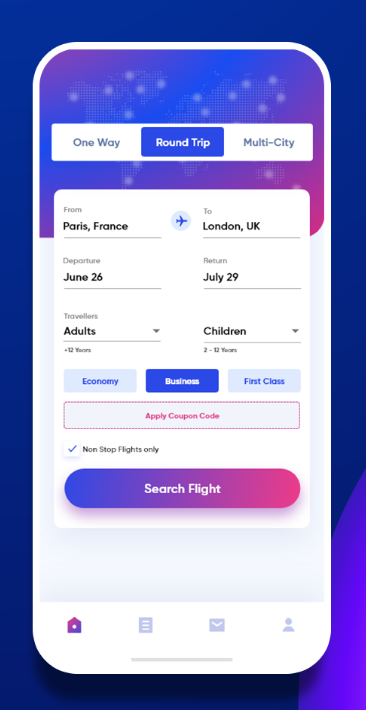
\includegraphics[scale=0.8]{img/info.png}
    \caption{Norimo skrydžio paieška}
    \label{img:info1}
\end{figure}
Šis interfeiso pavyzdys yra malonus akiai, jis patenkina pirminių siunteresuotųjų lūkesčius aiškiai ir greitai pasirinkti norimų skrydžių informaciją (Lūkestis Nr. \ref{itm:aisku}), bei antrinių suinteresuotųjų lūkečius prisijungti prie sistemos anonimiškai (Lūkestis Nr. \ref{itm:anonim}), nes į sistemą nereikia įvesti jokių asmeninių duomenų, kol bilietai nėra perkami.

\subsection{Datos pasirinkimas}
\subsubsection{Datos pasirinkimas kalendoriuje}
\begin{figure}[H]
    \centering
    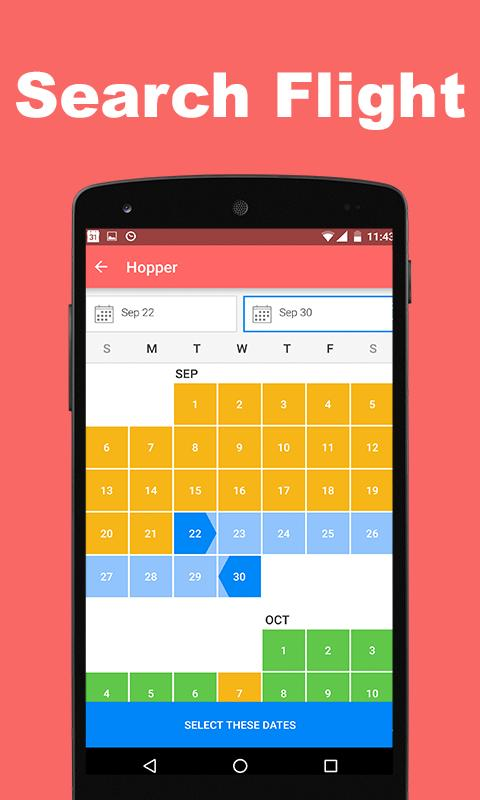
\includegraphics[scale=0.6]{img/hopper.jpg}
    \caption{Data1}
    \label{img:data1}
\end{figure}
Paspaudus ant išvykimo ir grįžimo datų gali pasirodyti kalendorius, toks, koks parodytas paveikslėlyje nr. \ref{img:data1}. Tai padėtų geriau suvokti visos kelionės, kurią vartotojas pasirinko, trukmę, patenkintų lūkestį aiškiai pasirinkti skrydžių datas (Lūkestis Nr. \ref{itm:aisku}).

\subsubsection{Data su vidutine kaina}
\begin{figure}[H]
    \centering
    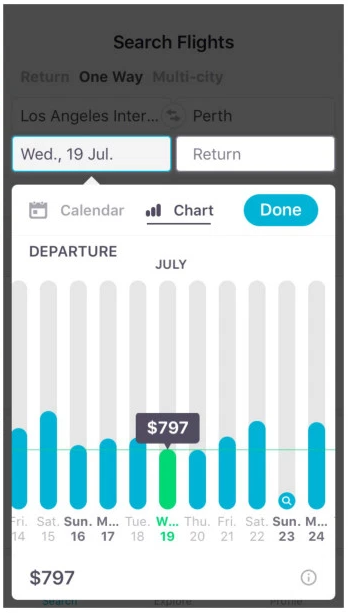
\includegraphics[scale=1]{img/skyscanner.png}
    \caption{Data2}
    \label{img:data2}
\end{figure}
Šis interfeiso pavyzdys patenkinta pirminių vartotojų lūkesčius greitai ir efektyviai rasti pigiausius bilietus (Lūkestis Nr. \ref{itm:pigu}), bei statistinių analizių vedėjų norą matyti bilietų kainas pagal datą dar būnant pradiniame sistemos lange- tam, kad būtų surinkti duomenys statistinei kainų analizei užtenka kelių paspaudimų (Lūkestis Nr. \ref{itm:analize}).

\subsection{Bilietų radimas}
\begin{figure}[H]
    \centering
    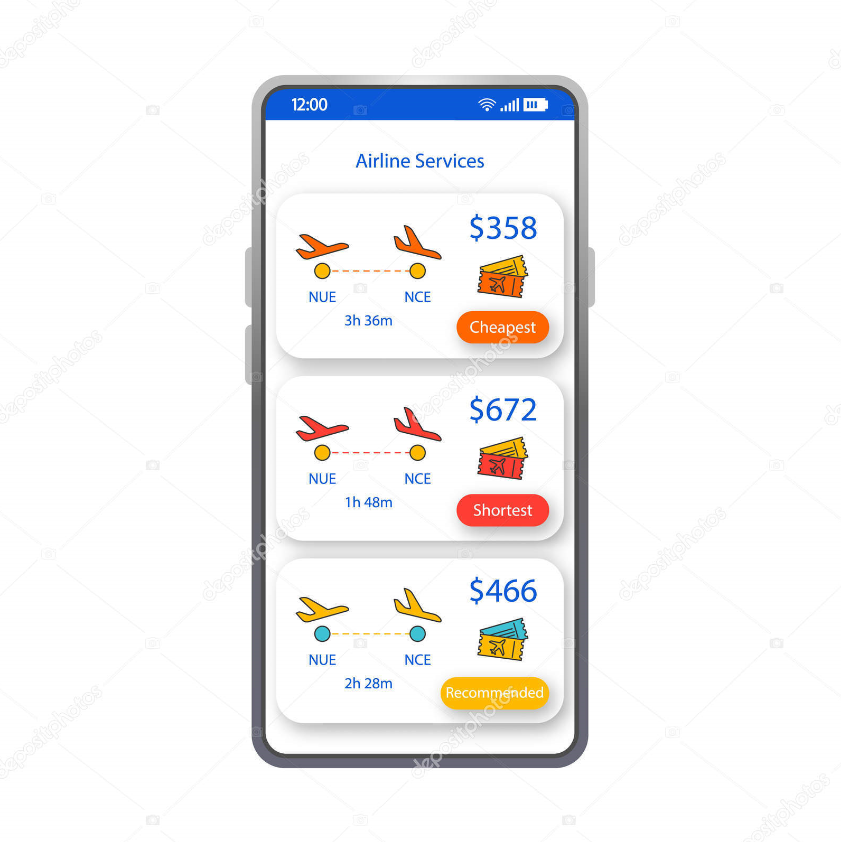
\includegraphics[scale=0.8]{img/deposit.png}
    \caption{Bilietų radimas}
    \label{img:radimas1}
\end{figure}
Šis dizainas leidžia aiškiai pamatyti sąrašą skrydžių norima data, taip pat yra atrinkti pigiausi, trumpiausi, bei rekomenduojami skrydžiai  (Lūkestis Nr. \ref{itm:aisku} ir  \ref{itm:pigu}). Dizainas yra gana minimalus, nėra elementų, kurie blaškytų vartotojo dėmesį, papildoma indormacija gali būti rasta paspaudus ant dominančio skrydžio. Tai palengvina pirminių suinteresuotojų veiklą sistemoje.

\newpage
\subsection{Turimų bilietų peržiūra}
\begin{figure}[htp]
\centering
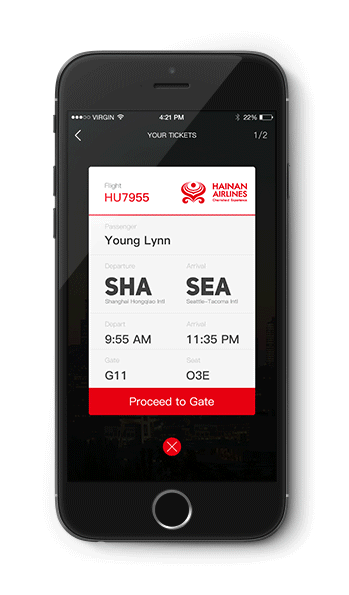
\includegraphics[width=.3\textwidth]{img/dribble1.png}\hfill
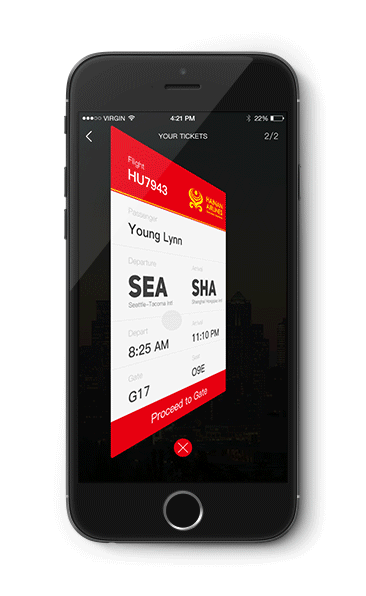
\includegraphics[width=.3\textwidth]{img/dribble2.png}\hfill
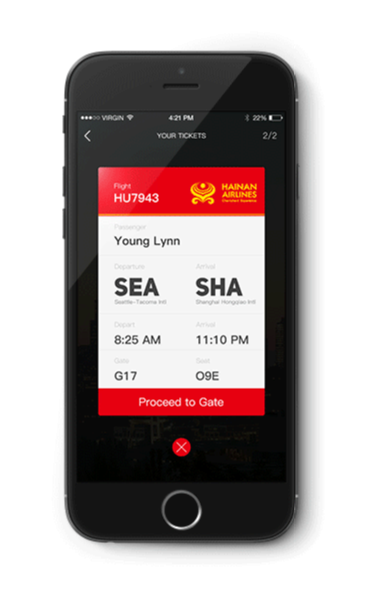
\includegraphics[width=.3\textwidth]{img/dribble3.png}
\caption{Bilietų peržiūra}
\label{fig:figure3}
\end{figure}
Šiame pavyzdyje vartotojas, atsidaręs išvykimo bilietą gali vienu braukimu į šoną pamatyti ir grįžimo atgal skrydžio bilietą. Tai patenkina keliautojų norą bilietus saugoti ilgą laiką, bei peržvelgti juos greitai ir patogiai (Lūkestis Nr. \ref{itm:aisku} ir \ref{itm:pigu}).

\printbibliography[heading=bibintoc, title=Šaltiniai]  % Šaltinių sąraše nurodoma panaudota
\end{document}
